\chapter[Automotive SPICE]{\thechapter. Automotive SPICE}
\section{Introduction}
With the rapidly increasing deployment of software based systems  in cars, the success of a product is strongly depended on quality of the supplied software. Thus leaving barely space for insufficiently and faulty designed software and requiring the need of an expert assessment during the design process of the software.\\
Automotive SPICE consists of two components, a process reference model and a process assessment model\footnote{See [Hoermann et al. 2006] for further details}. Comparing and evaluating of those two components gives standard possibility of making expert assessment any stage of the software design process.
\begin{center}
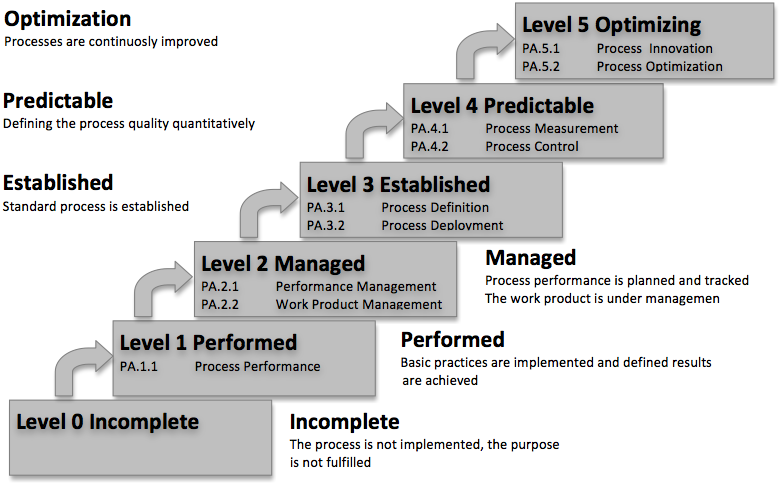
\includegraphics[scale=0.45]{Images/Automotive_Spice.png}\\
Figure 1.2 - The six levels\footnote{In order to make an assessment of a given level, the lower level shall be fully achieved. }
\end{center}
It would be beyond the intention of this project to try and cover all the process of Automotive SPICE.
\section{Software design process}
The main idea of software design process is to split the software into software components and provide a design that can be verified against the software requirements. This is done in a sequence of iterative steps, starting at the software architecture design,  until a detailed design is achieved.  The base practice that should be done are described in Goals and success criteria of project.